% prog-acos-cc-mc.tex

\documentclass[tikz]{standalone}
\usepackage{amsmath, amsfonts}
\usetikzlibrary{positioning, shapes, decorations.pathreplacing}

\newcommand{\acos}{$\textsl{COS}_{\mathcal{A}}$} % abstract causal operational semantics

\begin{document}
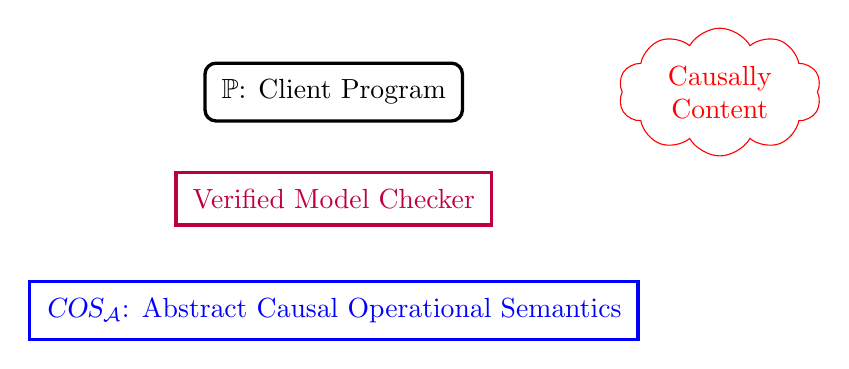
\begin{tikzpicture}[rect/.style = {draw, very thick, rectangle, inner sep = 6pt}, % rectangle
  rrect/.style = {rect, rounded corners}, % rounded rectangle
  cc/.style = {draw, cloud, cloud puffs = 10, cloud puff arc = 120, aspect = 2, 
  	inner xsep = 0.3em, inner ysep = 0.3em, align = center, red},
]
  \node (prog) [rrect] {$\mathbb{P}$: Client Program};
  \node (prog-cc) [cc, right = 2.0cm of prog] {Causally \\ Content};
  \node (abs) [blue, rect, below = 2.0cm of prog] {\acos: Abstract Causal Operational Semantics};

  % \pause
  \node (mc) [purple, rect, below = 1.0cm of prog.center] {Verified Model Checker};
\end{tikzpicture}
\end{document}
